\documentclass[11pt]{article}

\usepackage[margin=1in]{geometry}
\usepackage[T1]{fontenc}
\usepackage[utf8]{inputenc}
\usepackage{amsmath,amssymb}
\usepackage{booktabs}
\usepackage{tabularx}
\usepackage{array}
\usepackage{enumitem}
\usepackage{natbib}
\usepackage{xurl}
\usepackage{tikz}
\usetikzlibrary{arrows.meta,positioning,calc}
\usepackage[hidelinks]{hyperref}
\emergencystretch=3em

\title{When Does Structural Comparison Support Cognitive-Capacity Individuation?}
\author{Rintaro Sakamoto\\Independent Scholar, Kitakyushu, Japan}
\date{}

\newcommand{\Pin}{P_{\mathrm{in}}}
\newcommand{\Pout}{P_{\mathrm{out}}}
\newcommand{\Gsys}{G_{\mathrm{cog}}}
\newcommand{\World}{W}
\newcommand{\Coupling}{\Gamma}
\newcommand{\Experiment}{E_{\mathrm{exp}}}

\begin{document}
\maketitle

\noindent\textbf{Keywords:} cognitive ontology; structural comparison; cognitive capacities; pre-individuation; representation; philosophy of cognitive science


\begin{abstract}

Structural comparison can reveal genuine similarities across scientific claims without yet showing that those similarities individuate the same cognitive capacity. This paper argues that an inference from structural comparison to capacity identity is epistemically licensed only when the representation, preservation criterion, and granularity of the comparison are specified and independently warranted for that inferential use. The point is not merely that relevant structure should be justified. Successful reconstruction cannot non-circularly establish that the very distinctions made salient by the successful representation are identity-bearing. Beni's structural-realist program for theory integration provides the central positive target: even granting a fruitful common formalism, formal unification alone leaves open which invariants should carry individuative force. Two representation-sensitivity tests sharpen the burden. A lossless invertible refactorization shows that successful representation does not uniquely privilege one primitive factorization, while a deliberately lossy projection changes whether a conflict-monitoring claim and an episodic-memory claim count as sharing bounded structure. Further cases show that a shared historical label can lack a preserved structural bridge and that different labels can share bounded organization without thereby denoting one capacity. The literature corpus and replay analyses are used as diagnostic witnesses rather than prevalence estimates or substitutes for independent human coding. The result is a constraint on licensed identity inference, not a representation-neutral cognitive ontology.

\end{abstract}

\section{Introduction}

Cognitive science inherits a large vocabulary of capacities: memory, attention, learning, belief, skill, prediction, control, concepts, and many others. These labels are indispensable for communication and literature organization, but they can also acquire evidential force before the comparison that would justify that force has been made explicit. The same problem arises in the opposite direction when a formal framework reconstructs heterogeneous models successfully: representational unification can look like evidence of a shared capacity structure even when the relevant notion of sameness has not yet been stated.

The construct-validity tradition already denies that a construct validates itself by being named \citep{CronbachMeehl1955ConstructValidity,BorsboomMellenberghVanHeerden2004Validity}, and cognitive-ontology projects explicitly represent relations among concepts, tasks, and measurements \citep{PoldrackEtAl2011CognitiveAtlas,TurnerLaird2012CogPO,PoldrackYarkoni2016CognitiveOntologies}. The question here is narrower and more demanding: \emph{what must be true of a comparison before the resulting similarity or difference can count as evidence for capacity individuation?}

The paper's central thesis concerns epistemic entitlement rather than the existence of evidence in the abstract: \emph{An inference from structural comparison to cognitive-capacity identity is epistemically licensed only if the comparison representation, preservation criterion, and granularity are specified and warranted for that inferential use.} Specification is a transparency condition: a reader must be able to inspect what counts as preserved and what is allowed to disappear. Warrant is a further, non-circular condition: the identity relevance of the preserved structure cannot be supplied solely by the reconstruction success whose significance is under dispute. Here \emph{independent} means inferentially independent of that success, not necessarily statistically independent or drawn from a wholly separate dataset. Cognitive-capacity labels are at most prima facie guides to individuation, and the working basis is not claimed to be uniquely correct or representation-neutral.

The primary target is a reconstruction-to-identity inference: a move from successful unification or reconstruction within one representation to a claim about capacity identity before the identity relevance of the preserved structure has been warranted. Two derivative risks follow from the same problem. Historical labels can carry continuity into the conclusion without a structural bridge, and invariance observed within one representation can be promoted beyond the transformation class that generated it. The argument below focuses on the more basic inferential step and then uses the label-based and local-invariance cases as applications.

The issue is live in recent work on cognitive ontology, scientific representation, and kind individuation. The next section therefore reconstructs the strongest relevant form of structural-invariance reasoning---with Beni as the central positive interlocutor---before turning to the diagnostic analyses.

The direct analytical objects are source-grounded \emph{scientific claims about cognitive capacities}. The inferential relation is therefore
\[
\begin{gathered}
\text{claim-level structural comparison}\\
\Downarrow\\
\text{evidential constraint on capacity comparison}\\
\Downarrow\\
\text{capacity individuation}.
\end{gathered}
\]
Most of the analysis concerns the first arrow. One downstream semantic-memory application is then carried further: it shows how the procedure changes the status of an actual capacity-level grouping from label-supported continuity to an open thesis carrying explicit preservation debt.

The method suppresses historical construct labels and selected source-authority metadata at the comparison stage, preserves the failure of an initially over-discriminating whole-claim comparison, asks a separately declared bounded-reuse question, reverse-projects the surviving structure into a compact role grammar, and tests representation sensitivity and prospective reconstruction. The procedure is therefore \emph{construct-label-suppressed at the comparison stage}, not theory-neutral or representation-neutral.

Figure~\ref{fig:pipeline} summarizes the reconstruction sequence. Its important feature is not the amount of audit machinery but the separation of comparison questions: a failure at one granularity is retained rather than silently relaxed, and a success under one representation is not automatically promoted to representation-independent identity.

\begin{figure}[htbp]
\centering
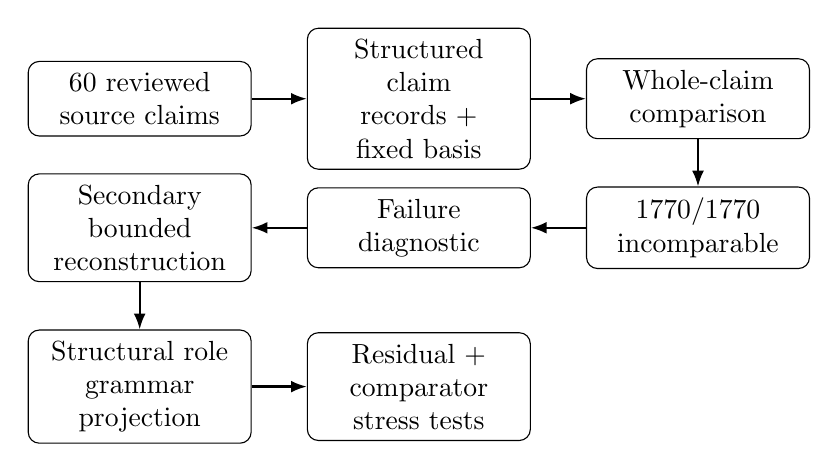
\begin{tikzpicture}[
  node distance=6mm and 7mm,
  box/.style={draw, rounded corners, align=center, inner sep=4pt, text width=2.55cm},
  arrow/.style={-{Latex[length=2mm]}, thick}
]
\node[box] (source) {60 reviewed\\source claims};
\node[box, right=of source] (records) {Structured claim\\records + fixed basis};
\node[box, right=of records] (phi) {Whole-claim\\comparison};
\node[box, below=of phi] (fail) {\(1770/1770\)\\incomparable};
\node[box, left=of fail] (diag) {Failure\\diagnostic};
\node[box, left=of diag] (arch) {Secondary bounded\\reconstruction};
\node[box, below=of arch] (grammar) {Structural role\\grammar projection};
\node[box, right=of grammar] (stress) {Residual +\\comparator stress tests};
\draw[arrow] (source) -- (records);
\draw[arrow] (records) -- (phi);
\draw[arrow] (phi) -- (fail);
\draw[arrow] (fail) -- (diag);
\draw[arrow] (diag) -- (arch);
\draw[arrow] (arch) -- (grammar);
\draw[arrow] (grammar) -- (stress);
\end{tikzpicture}
\caption{Reconstruction sequence. Whole-claim failure is preserved and diagnosed before the secondary bounded-subobject reconstruction.}
\label{fig:pipeline}
\end{figure}


\section{From reconstruction success to licensed identity inference}

Three questions must be kept apart. First, a comparison must be \emph{specified}: its representation, preservation criterion, and granularity must be explicit enough to determine what counts as sameness and what may disappear. Second, those choices must be \emph{warranted for the identity inference}: there must be a reason to treat the preserved structure as relevant to the capacity boundary at issue. Third, the observed comparison result must actually support the particular capacity-level conclusion being drawn.

The second requirement is the central philosophical claim. The argument can be stated directly:

\begin{enumerate}[leftmargin=*]
\item Successful reconstruction under a representation \(R\) establishes an achievement relative to \(R\): the source claims can be encoded, related, or unified while preserving the distinctions that \(R\) declares relevant.
\item An inference to cognitive-capacity identity requires more than reconstructability. It requires that the preserved distinctions be identity-relevant at the capacity granularity under discussion.
\item Reconstruction success under \(R\) cannot, by itself, non-circularly establish that identity relevance. Otherwise the same success both selects the comparison dimensions and certifies that those dimensions individuate the capacity.
\item Rival representations can preserve reconstructability while changing which distinctions are primitive, and controlled information loss can change whether two claims count as sharing structure.
\item Therefore successful structural reconstruction alone cannot determine which represented invariance is identity-bearing. A further bridge principle or independent warrant is required.
\end{enumerate}

This is stronger than the generic advice that one should compare only relevant features. It identifies a specific inadmissible source of justification: the relevance of the preserved structure cannot be supplied solely by the reconstruction success whose significance is in question.

The burden can be discharged in more than one way. A mechanistic argument may show that the preserved organization constitutes the phenomenon; a causal argument may identify capacity-relevant difference-makers; a cross-context or intervention-sensitive invariance argument may show that the same organization remains stable under independently motivated changes; an explanatory argument may show that the preserved structure carries the relevant explanatory work; and an objective-perspicuity argument may show that one representation is better aligned with the target structure. These routes need not use statistically independent data. What they must not do is merely redescribe reconstruction success as its own warrant.

The empirical analyses below therefore function principally as diagnostics of this inferential burden. Scientific-representation theory supplies the broader background: representational equivalence and surplus structure depend on what a mapping preserves \citep{Nguyen2017RepresentationEquivalence,NguyenTehWells2020Surplus,FriggNguyen2020ModellingNature,NguyenFrigg2022ScientificRepresentation}.

\section{Structural invariance as a live target}

Beni's structural-realist proposal for consciousness science provides the clearest contemporary target \citep{Beni2026KindsWithoutStructure}. The strongest charitable reconstruction of that proposal is not that any successful formalization automatically reveals a natural kind. Rather, a common formal framework can expose relational invariants across otherwise heterogeneous theories, and those invariants may in turn support theory integration and kind individuation. The present argument grants the first step. A common representation can genuinely reveal stable relational organization.

The pressure point is the second step: \emph{what makes the revealed invariance identity-bearing rather than merely representationally salient?} Even if predictive processing or the free-energy framework is an excellent unifying basis, successful unification alone does not settle which invariant should individuate the relevant kind or cognitive capacity. The conditional challenge is therefore: if structural invariance is to do individuative work, the proposal must also explain why the representation, transformation class, and granularity that expose that invariance preserve what matters for identity. This is not an attribution of a simple fallacy to Beni. It is an additional burden that arises when formal unification is asked to support individuation.

Wajnerman-Paz and Rojas-L\'ibano sharpen the same issue from cognitive ontology by making across-context invariance central to simultaneous individuation of mechanisms and capacities \citep{WajnermanPazRojasLibano2026Bidimensional}. Their proposal gives a substantive answer to the question \emph{which stability should matter?}: stability across scientifically relevant contexts can constrain both sides of the mechanism--capacity relation. The present contribution is prior and complementary. It asks how the relevant contexts, transformations, preservation relation, and granularity are selected and why that selection tracks identity rather than convenience.

North's defense of objective or non-pragmatic perspicuity shows one way the burden could be met \citep{North2026Perspicuous}. If a representation can be shown, independently of its success at accommodating the present cases, to display the target structure more perspicuously than its rivals, then that argument supplies precisely the sort of bridge warrant required here. The burden principle is therefore not a thesis that every representation is equally interest-relative. It is compatible with a successful realism about perspicuity; it simply requires that the perspicuity argument do work that reconstruction success cannot do by itself.

Brousalis makes epistemically relevant similarities and differences central to theory comparison \citep{Brousalis2026TheoryComparison}. The present claim adds a non-circularity constraint to that insight. It is not enough that a similarity be declared relevant to the comparison; when the comparison is used to support individuation, the relevance of the similarity cannot be inferred solely from the fact that the chosen representation reconstructs the cases successfully. Francken, Slors, and Craver, Krickel, and Koh\'ar likewise show why abstraction, operationalization, mechanism, and system-boundary choices must remain tied to explanatory practice rather than silently hardening into a taxonomy \citep{FranckenSlorsCraver2022CognitiveOntology,Krickel2024CognitiveOntology,Kohar2025ScalingUp}.

The paper therefore targets a \emph{reconstruction-to-identity inference}: a move from successful structural reconstruction to a conclusion about capacity identity before the identity relevance of the preserved structure has been independently warranted. Terminological continuity and local invariance are important derivative risks, but the central issue is the bridge from reconstruction success to individuation.

\section{Methods}

\subsection{Designed corpus}

The bounded empirical target contains 60 claims. Forty-eight primary claims are divided evenly across eight historical construct strata. Twelve additional claims form a non-tuning challenge surface.

\begin{table}[htbp]
\centering
\caption{Designed corpus. The corpus is a stress-test surface, not a probability sample or prevalence estimator.}
\label{tab:corpus}
\begin{tabular}{lrr}
\toprule
Surface & Design & Claims \\
\midrule
Primary & 8 strata \(\times\) 6 claims & 48 \\
Challenge & 12 predeclared pressure classes & 12 \\
\midrule
Total & & 60 \\
\bottomrule
\end{tabular}
\end{table}

The primary strata are Memory, Learning, Skill, Attention, Prediction, Control, Belief, and Concept. Challenge pressures include multi-timescale organization, stochastic or approximate structure, constitutive boundary pressure, compositional or systematic structure, embodied or world-coupled organization, normative or criterion structure, hybrid labels, label-coordinate mismatch, multi-condition structure, same-inventory/different-topology pressure, strict-refinement pressure, and high structural heterogeneity. Challenge claims were not permitted to tune the structured-record schema, working basis, or comparison semantics.

This is a literature-based structural comparison, not an experiment or prevalence study. Its role is instead adversarial and structural: the 48 primary claims provide balanced coverage across historically familiar construct strata, while the 12 challenge claims probe predeclared pressures that could break the representation. Consequently, the supported inference is whether reusable structure survives this designed stress-test surface under pre-specified rules, not how prevalent any role or reusable structural subobject is in cognitive science as a whole.

\subsection{Source-grounded structured claim records}

Each selected source claim was represented in a machine-readable structured claim record containing stable source identity, source-local evidence locators, claim scope and modality, typed nodes, typed relations, temporal information, control information, approximation state, and bridge assumptions.

A language model assisted initial structured extraction, but its output was not treated as authority. Every retained record was reviewed against source text, and all 60 current records carry reviewed status. The scientific input to downstream analysis is therefore the source-audited structured claim corpus.

Independent extraction reliability was not established. Historical local two-pass calibration transactions produced zero valid structured claim records in both the v2 and v3 real calibration runs, leaving no valid A/B agreement denominator. The present study consequently claims auditability of the retained corpus, not inter-model agreement, autonomous extraction reliability, or deterministic language-model replay.

\subsection{Pre-specification and anti-circularity}

The comparison basis, whole-claim projection, and bounded-reconstruction rules were fixed before later grammar and prospective outcomes were used to interpret them. Reverse projection did not reread source papers or rewrite the reviewed claim records to improve grammar coverage, and residuals were retained rather than repaired after inspection. The purpose of this staging is not to remove author judgment, which remains present in source review and structural adjudication, but to prevent the final grammar from simultaneously defining and validating its own input representation. Exact repository chronology, immutable hashes, and stage-level provenance are reported in the Supplementary Methods rather than used as argumentative premises in the main text.

\subsection{Generative AI and human accountability}

OpenAI ChatGPT assisted structured extraction, source-analysis workflow, software development, and manuscript drafting. Model output was not treated as source authority or as an independent adjudicator. Every retained claim in the 60-claim reference corpus was reviewed by the author against source text, and the prospective study tied adjudications to explicit source locations and versioned artifacts. Independent extraction reliability and independent human re-adjudication were not established; these remain distinct limitations. Full disclosure and workflow provenance are provided in the Supplementary Methods.

\subsection{Pre-specified structural basis}

The structural comparison suppresses source information that should not determine similarity merely by appearing in a paper. Author identity, institution, venue, citation count, historical construct label, source-local identifiers, and free-text presentation are excluded from comparison.

The pre-specified working basis is
\[
B_{P2}=\{S,\Pi,K,O,T,C,Q,P\},
\]
interpreted as a declared structural coordinate system for comparison rather than an ontology or a representation-neutral basis. Lexical shortcuts are forbidden: a source node named \emph{condition} is not automatically \(C\); a reward-like term does not exhaust \(Q\); temporal precedence is not automatically \(K\); and a partition need not be physical.

\subsection{Whole-claim comparison}

The pre-specified \(\Phi\) projection preserves claim type, modality, scope shape, typed topology, active basis coordinates, temporal presence states, control states, approximation mode, and bridge-grounding multiplicity. It forgets source authority and presentation metadata.

Pairwise relations distinguish equivalence, refinement, forgetting, incomparability, and mutual-embed non-isomorphism. For 60 claims, the unordered comparison surface contains
\[
\binom{60}{2}=1770
\]
pairs.

\subsection{Secondary bounded reconstruction}

Because whole-claim comparison failed universally, the next analysis changed the \emph{unit of reuse}, not the pre-specified source representation. The whole-claim result therefore remains the primary result for the original \(\Phi\)-level question. A secondary post-atlas reconstruction then asked a different question: whether bounded substructures could recur even when complete scientific claims remained incomparable. In that chronological sense the reconstruction is post-atlas; it is not presented as if it had been the successful primary comparison from the outset.

The bounded reconstruction searched for basis-subobjects recoverable under a pre-specified forgetting operator. The operator permits restriction to retained typed substructure but forbids arbitrary rewiring and semantic relabeling. Thus the secondary analysis does not revise the 1,770 whole-claim verdicts, and successful bounded recurrence cannot be used to retrospectively relabel a failed whole-claim pair as equivalent.

Negative and ablation controls tested trivial-core collapse, label dependence, permissive forgetting, richer competing cores, overlapping incomparable cores, cross-label recurrence, compatibility with whole-claim incomparability, and presentation invariance. No post-outcome abstraction threshold was added to manufacture recurrence.

\subsection{Structural role grammar and adversarial tests}

Surviving bounded structures motivated a compact structural role grammar (version 0):
\[
\Gsys=\{\Pi,X,C,Q,\Pin,\Pout,K,T,\rho/O\}.
\]
Here \(X\) is a generic configuration carrier; \(C\) is realizability/admissibility structure; \(Q\) is criterion-conditioned orientation; \(\Pin\) and \(\Pout\) are directional interface roles; \(K\) is typed transformation or dependence; \(T\) is succession or temporal indexing; and \(\rho/O\) is boundary-relative observation or trace.

A mnemonic representation is
\[
X_{n+1}=K_{n;C,Q,\Pin}(X_n),
\qquad
O_n=\rho_{\Pi,C,\Pout,n}(X_n),
\]
without assuming that every claim instantiates every role.

All 60 reviewed claims were reverse-projected into this structural role grammar without rereading source papers or changing the structured claim records, \(B_{P2}\), \(\Phi\), structural adjudications, or reusable-subobject identities. Residuals were classified under a pre-specified taxonomy in which only an unexplained requirement for an additional top-level system role counted as prima facie evidence for extending the role inventory.

Two strict distinction-preservation comparators were tested:
\[
G_{\mathrm{dyn}}=\{X,K,T\},
\qquad
G_{\mathrm{pomdp}}=\{X,P,K,\rho/O,Q,T\}.
\]
These are distinction-loss tests, not non-encodability theorems.


\subsection{Prospective non-selection control}

After the original 60-claim analysis and role grammar were fixed, a separate no-substitution roster of 40 cognitive-model papers was reconstructed under the same source-faithful criteria. All 40 could be reconstructed without adding a new coordinating mechanism beyond what the source model itself specified. This remains a source-grounded, single-adjudicator finding; DOI separation from the original corpus is not treated as genealogical independence.

For the present argument, the important result is negative. The same 40 papers also remain reconstructable under six weaker encoding-capable views. Successful direct reconstruction therefore does not select the exact role inventory. When the criterion is strengthened so that omitted distinctions must remain directly available rather than being reintroduced by an adapter, all six weaker views incur preservation debt. The two tests answer different questions and are reported in full in the Supplementary Methods. Their philosophical role is simply to separate reconstructability from representational privilege.

\subsection{Lossless non-uniqueness and a genuinely lossy rival representation}

Two different representation-sensitivity questions are kept separate. First, an invertible Tagged Admissibility--Interface Factorization (TAIF) tests whether the exact nine first-class roles are unique when the same information is losslessly refactored. Second, a Coarse Process--Constraint Graph (CPCG) asks whether higher-order bounded-reuse conclusions survive a deliberately information-losing representation.

CPCG has five coarse families: \(N\) for carrier/component structure, merging state-like and partition/boundary structure; \(G\) for guard/orientation, merging constraints and criteria; \(I\) for interface events, merging probes/interventions with observations/readouts; \(E\) for non-temporal transformation/dependence; and \(T\) for temporal presence/order. Fine node-role strings, working-basis control subtypes, non-temporal relation kinds, and detailed temporal subtypes are discarded. The map is therefore non-injective by construction. No retention threshold was declared: survival and collapse are both reportable sensitivity outcomes.


\subsection{Epistemic status of the reported results}

The corpus is a designed diagnostic surface, not a probability sample. Exact counts are therefore reported for auditability but are not treated as prevalence estimates or as the philosophical contribution itself. The main inferential roles are summarized in Table~\ref{tab:epistemic-status}.

\begin{table}[htbp]
\centering
\caption{Epistemic status of the principal analyses.}
\label{tab:epistemic-status}
\begin{tabularx}{\textwidth}{>{\raggedright\arraybackslash}p{0.30\textwidth} >{\raggedright\arraybackslash}p{0.22\textwidth} >{\raggedright\arraybackslash}X}
\toprule
Analysis & Status & Licensed use \\
\midrule
Whole-claim comparison & Representation diagnostic & Shows that the specified whole-claim comparison is too discriminating for the intended reuse question. \\
Bounded structural reuse & Source-grounded diagnostic & Supplies concrete witnesses of recurrent bounded organization conditional on the reviewed records and forgetting rule. \\
Role-grammar projection & Source-grounded audit & Tests how much of the reviewed corpus is expressible in the compact role vocabulary; it does not establish that this vocabulary is uniquely correct. \\
Prospective 40-paper reconstruction & Secondary non-selection control & Shows that successful reconstruction does not privilege the exact working basis. \\
Lossless and lossy representation tests & Representation diagnostic & Test whether first-class factorization and overlap judgments survive controlled changes of representation. \\
Constructed perturbations & Reachability control & Confirm that the comparison procedure can return alternative outcomes under source-derived counterfactual damage. \\
Worked cases & Philosophical witnesses & Make the inferential burden concrete; they do not estimate population frequencies. \\
\bottomrule
\end{tabularx}
\end{table}

\section{Results}

\subsection{Whole-claim comparison diagnoses excessive granularity}
\label{sec:wholefail}

The pre-specified whole-claim comparator classified all 1,770 unordered pairs as incomparable. In the corresponding 3,540 directed comparisons, 3,518 stopped at the scalar stage, six reached node-count comparison, 16 reached node-label multiset comparison, and none reached topology or embedding.

The philosophical use of this result is therefore diagnostic rather than triumphalist. The rich whole-claim representation distinguishes the corpus so early that it supplies almost no reusable equivalence structure. Universal incomparability is retained because it identifies a failed comparison granularity; it is not presented as evidence that cognitive capacities are globally incommensurable or that graph topology separates every claim.

\subsection{Comparator reachability controls}

The universal whole-claim incomparability result raises an immediate sanity question: can the comparator ever return a positive relation? Three pre-specified constructed controls answer this without adding corpus evidence. An identifier/presentation renaming of the same structural claim returns \textsc{equivalent}. A presentation-only metadata variant, changing source-facing metadata that the pre-specified projection explicitly forgets while leaving scientific structure untouched, also returns \textsc{equivalent}. Finally, adding one authorized fixed resource distinction returns \textsc{right-strict-refinement-of-left}, with the forgotten \(C\) axis and resource control recorded in the witness. These are \emph{CONSTRUCTED\_CONTROL} results. They establish reachability of equivalence and refinement states under the comparator; they do not validate a cognitive taxonomy or weaken the held-fixed \(1770/1770\) corpus result.

\subsection{Bounded reusable structure reappears}

The secondary bounded reconstruction produced 213 within-stratum candidate subobjects and 206 unique reusable structural subobjects. Seven exact cross-stratum equivalence components survived. The global refinement structure contains 470 direct refinement edges and 2,894 strict subobject relations in transitive closure.

The bounded family structure contains
\[
99\ \text{cross-stratum families}
\qquad\text{and}\qquad
107\ \text{within-stratum-only families},
\]
with 188 distinct support signatures. Fifty-nine of 60 claims are covered by at least one surviving bounded object. All eight negative and ablation controls pass.

Notably, 1,304 whole-claim pairs share at least one surviving reusable structural subobject despite every whole-claim pair being held as incomparable. Whole-claim identity and reusable substructure are therefore distinct questions on the same corpus.

\subsection{Reverse projection is secondary to the identity argument}

Reverse projection of the 60 reviewed claims into the compact role grammar yields 21 FULL, 22 PARTIAL, and 17 RESIDUAL cases. None of the 17 residuals requires a new top-level role under the held-fixed adjudication. These results remain useful as an audit of the working representation, but they are not evidence that the exact role inventory is uniquely correct. Detailed role frequencies, residual classes, and strict distinction-preservation comparator results are therefore moved to the Supplementary Methods rather than treated as first-class philosophical results.

\subsection{Critical representation-sensitivity tests}

The first test is lossless. The invertible refactorization used here preserves the information needed to reconstruct the original role structure while changing how that structure is factored. Successful representation therefore does not uniquely privilege the original first-class inventory: lossless recoding can preserve scientific content while changing which distinctions appear primitive.

The second test is deliberately lossy. Under the fine bounded representation, the conflict-monitoring claim reconstructed from Botvinick et al. and Tulving's episodic-memory claim share no exact bounded object \citep{BotvinickEtAl2001ConflictMonitoring,Tulving2002EpisodicMemory}. A coarser projection deliberately forgets the difference between two temporal-state organizations and causes them to collapse to the same coarse signature. The pair therefore moves from zero overlap to positive overlap under the coarser representation.

No new control--memory capacity follows from that collapse. The point is methodological: whether the two claims count as sharing structure depends on the preservation contract. If the forgotten temporal distinction is identity-relevant, the coarse representation over-unifies the pair; if it is irrelevant to the capacity question, the coarse overlap may be useful. Reconstruction success cannot decide between those interpretations.

Together, the lossless and lossy tests do more than show that representations differ. They identify why reconstruction success cannot self-certify identity relevance. The lossless test shows underdetermination of primitive factorization even without information loss; the lossy test shows that an overlap judgment itself can change when preservation is weakened. A bridge principle is therefore required before the invariance exposed by a representation can bear individuative weight.

\subsection{Secondary prospective control}

The separate 40-paper study supports the same negative conclusion from another direction. All 40 sources remain directly reconstructable under the working basis and under six weaker encoding-capable views. When direct preservation of the omitted distinctions is required, those weaker views incur preservation debt. This is not the paper's primary evidence for the burden principle; it is a non-selection control showing that generic reconstructability and representational privilege are different achievements. Full classifications and paper-level provenance are reported in the Supplementary Methods.

\subsection{Validation diagnostics: separating claim selection from decomposition}

A blinded source-reconstruction replay initially allowed each model configuration to choose one focal claim from each source. That design produced many apparent disagreements with the retained reference, but inspection showed that the replay and the reference were often reconstructing different claims from the same paper. The validation task had therefore confounded \emph{claim selection} with \emph{claim decomposition}.

A second, prospectively specified replay fixed the focal claim in advance by supplying a source locator and a minimally identifying proposition while continuing to withhold the retained structural answer. Under that design, each of two independently run named-model configurations produced a structurally compatible alternative to the retained reconstruction in nine of ten cases, and the two replay configurations were mutually compatible in all ten. None reproduced the exact first-class factorization. The remaining retained-reference disagreement concerned the timing description in Karpicke and Blunt's retrieval-practice study \citep{KarpickeBlunt2011RetrievalPractice}. Correcting that source-level statement changed semantic provenance but, under deterministic sensitivity analysis, left the whole-claim comparison, bounded reuse, and role-projection results unchanged.

These replay analyses are secondary validation diagnostics, not independent human coding, not cross-provider replication, and not evidence of unseen-source generalization. Their relevance to the philosophical argument is narrower: once the claim being reconstructed is held fixed, identity-relevant dependencies can be reproducible even when exact representational factorization remains non-unique. Detailed model provenance, scoring rules, case-level outcomes, and correction records are reported in the Supplementary Methods.

\section{Capacity-level consequences}

\subsection{Different labels can share bounded organization}

Duncan's work on object-based visual attention and Behrens et al.'s work on volatility-sensitive learning begin under sharply different historical labels \citep{Duncan1984SelectiveAttention,BehrensEtAl2007ValueInformation}. Their complete structured claims remain incomparable. At a separately declared bounded granularity, however, both instantiate the same general organization: a probe maps to an outcome through typed conditional structure. Because construct labels are excluded from the comparison, this is not a lexical match.

The inference stops there. Their fuller role profiles differ, and their complete claims remain incomparable. The licensed conclusion is therefore asymmetric: label difference does not by itself justify a capacity split, and recurrent bounded organization gives a reason to investigate a cross-label bridge; but one shared substructure does not establish whole-capacity identity. That stronger inference requires an argument that the shared organization is identity-relevant at the capacity granularity in question.

\subsection{A shared label need not supply the bridge}

Tulving's episodic-memory analysis and Patterson, Nestor, and Rogers' account of semantic/conceptual knowledge both sit near the historical label \emph{semantic memory}, but the label plays different roles in the two source claims \citep{Tulving2002EpisodicMemory,PattersonNestorRogers2007Semantic}. In Tulving's analysis, the primary target is a past-oriented episodic subsystem, with a knowledge-oriented subsystem entering as a contrast and dependence. In Patterson et al., semantic/conceptual knowledge is itself the direct target of an architectural claim involving distributed representations, convergence, and cross-modal generalization.

The bounded structural supports of the two claims are disjoint under the fine representation and remain disjoint under the tested coarse projection. This does \emph{not} show that semantic memory is not one capacity. It changes the evidential status of that thesis: recurrence of the label no longer supplies the required bridge by itself.

A unified semantic-memory thesis would therefore need additional evidence that aligns the targets of the two descriptions, states the granularity at which their organizations are to count as evidence about the same capacity, specifies what is preserved across the bridge, and explains why the chosen representation is appropriate for the identity question. The capacity thesis remains open, but the preservation debt is explicit.

\subsection{Representation choice can change the existence of overlap}

The Botvinick et al.--Tulving comparison provides the clearest representation-sensitive boundary case \citep{BotvinickEtAl2001ConflictMonitoring,Tulving2002EpisodicMemory}. Under the fine bounded representation, the conflict-monitoring claim and the episodic-memory claim share no exact bounded object. One preserves persistence with a time index; the other preserves a history window with a time index. The fine comparison keeps those temporal organizations distinct.

The deliberately coarse projection forgets that distinction, so the two temporal-state objects collapse to the same signature and the pair acquires positive overlap. This is not evidence for a newly discovered control--memory capacity. It shows that the sentence \emph{these claims share structure} can change truth value when the preservation contract changes. The capacity-level question is therefore not whether overlap can be produced, but whether the preserved equivalence is warranted as identity-relevant.

\section{Worked example: from source evidence to a capacity constraint}

The Duncan--Behrens comparison can be followed through the complete analysis without consulting the repository. Duncan's source evidence relates report accuracy to whether attributes belong to the same or different perceptual units; Behrens et al. relate outcome history and inferred environmental change to subsequent choice \citep{Duncan1984SelectiveAttention,BehrensEtAl2007ValueInformation}. The structured records preserve those source-specific organizations before any bounded comparison is attempted.

At the whole-claim level, the two organizations are incomparable. The analysis then changes the question rather than changing that verdict: under the separately declared bounded forgetting rule, both instantiate the same probe-to-outcome organization with typed conditional dependence. That organization also recurs elsewhere in the corpus, so it is not an ad hoc resemblance invented for this pair.

Restoring the surrounding structure reintroduces the differences. The licensed inference is therefore that differently labelled attention and learning claims can reuse a bounded organization, so label difference alone cannot justify a capacity split and a cross-label identity hypothesis deserves further investigation. What is not licensed is the stronger claim that object-based attention and volatility-sensitive learning are one capacity. That requires further warrant that the shared organization is constitutive or otherwise identity-relevant at the chosen capacity granularity.

\section{Boundary conditions on the comparison}

The comparison does not supply a universal criterion for where a cognitive system ends. Internal transformation, cross-boundary coupling, and experimental scheduling are kept distinct so that an experimental condition or environmental state is not silently promoted to an internal cognitive role. System boundaries therefore remain application-relative, a point compatible with dynamical, embodied, enactive, and extended approaches. The explicit system--environment--experiment typing and the treatment of experiment start as a cut through a longer history are preserved in the Supplementary Methods.

\section{What could discharge the warrant?}

The closest philosophical relations are not merely precedents; they identify different ways the evidential burden might be discharged or resisted.

Francken, Slors, and Craver distinguish operationalization, abstraction, and boundary problems in cognitive ontology \citep{FranckenSlorsCraver2022CognitiveOntology}. The present procedure does not solve those problems. It makes one consequence explicit: a capacity-to-mechanism or capacity-to-claim comparison cannot borrow its identity criterion from the vocabulary whose individuation is in question. Wajnerman-Paz and Rojas-Líbano make across-context invariance central to simultaneous individuation of mechanism and capacity \citep{WajnermanPazRojasLibano2026Bidimensional}. The present contribution does not compete with that criterion; it identifies a prior evidential condition on its use. A claim of invariance must specify the representation, the relevant context or transformation class, the preservation relation, and the granularity at which stability is assessed, and those choices must be warranted for the identity inference rather than selected merely because they generate stability.

Beni's structural-realist proposal is a more direct positive foil \citep{Beni2026KindsWithoutStructure}. Beni uses predictive processing as a candidate formal basis for identifying invariant relations across divergent consciousness theories. The present results do not show that such a basis is wrong. They show why \emph{successful unification by itself} is insufficient as identity evidence: the prospective 40-paper set remains directly reconstructable under multiple weaker encoding-capable views. A candidate unifying representation therefore requires an additional reason for privileging the structure it makes first-class---for example, a justified preservation criterion, independent empirical invariance, or a perspicuity argument.

That last possibility connects the paper to North. North argues that some representations in physics can be objectively and non-pragmatically more perspicuous than alternatives \citep{North2026Perspicuous}. The present study does not adopt the contrary view that all representations are merely purpose-relative conventions. Instead it separates two questions: what follows from a declared preservation purpose, and whether one representation is independently better aligned with the target. CPCG and TAIF address the first question by exposing sensitivity and non-uniqueness; they do not settle the second. If the working basis is objectively more perspicuous, that requires an argument beyond its ability to encode the corpus.

Brousalis emphasizes that theory comparison depends on identifying similarities and differences that are epistemically relevant to the purpose of comparison \citep{Brousalis2026TheoryComparison}. The present preservation contract makes one such relevance decision inspectable rather than tacit. Onishi and Serpico, by contrast, show why causal and structural category boundaries may remain interest-relative \citep{OnishiSerpico2022HPC}. That warning remains in force here: selecting a system boundary, granularity, or preservation criterion is an inquiry-relative methodological act. The proposed remedy is disclosure and sensitivity analysis, not the discovery of a purpose-independent taxonomy.

Krickel's analysis reinforces the same boundary from a different mechanistic direction: mechanisms can be epistemically useful without mechanically determining the correct capacity taxonomy \citep{Krickel2024CognitiveOntology}. Koh\'ar's concrete treatment of scaling-up likewise illustrates why the relevant philosophical dispute should be tied to what explanatory organization a mechanism actually supplies rather than to a binary allegiance between formalisms \citep{Kohar2025ScalingUp}.

The method is therefore neither a replacement cognitive ontology nor a theory of representational perspicuity. It is a constraint on when structural comparison may be used as evidence in those stronger projects.

\section{Limitations and validation boundary}

The corpus is purposive and diagnostic. It is not a probability sample, so neither the frequency of structural roles nor the frequency of prospective reconstruction outcomes should be interpreted as population prevalence. The exact counts are useful for auditability and for locating counterexamples, but the philosophical argument depends primarily on the existence of the representation-sensitivity witnesses.

Independent human re-adjudication was not performed. The retained source records were reviewed against source text, and the model replays provide a separate procedural check, but neither substitutes for independent human coding. Procedural auditability is established; inter-rater reliability remains unmeasured.

The modeled system boundary is application-relative rather than a discovered universal cognitive boundary. Structural typing helps prevent internal transformation, environmental coupling, and experimental scheduling from being silently conflated, but it does not determine which boundary every scientifically appropriate theory must adopt.

Only one deliberately lossy rival representation is used in the central sensitivity test. Together with the lossless refactorization, this is enough to show that reconstruction success does not uniquely fix primitive factorization and that overlap can change under controlled information loss. It is not enough to establish representation neutrality or to show that every reasonable rival representation produces the same pattern.

The prospective 40-paper analysis is a non-selection control, not an independent random holdout. The papers were purposively chosen for architectural coverage, and the analysis does not support binomial significance or population inference. Its role is limited to showing that successful reconstruction persists under weaker encoding-capable views and therefore cannot by itself privilege the full working basis.

The formal verification checks declared typing, dependencies, and transformation rules. It is an audit layer rather than an empirical validation layer: it can expose inconsistent formal commitments but cannot establish empirical adequacy, cognitive truth, or a uniquely correct ontology.

Finally, the claim-anchored replay was designed after the initial unanchored replay exposed a claim-selection confound. It is therefore prospective relative to its own outputs but not independent confirmation of the earlier diagnosis. The resulting same-source compatibility is informative about decomposition reproducibility under the tested conditions, not about unseen-source generalization, provider independence, or human reliability. The subsequent source correction was kept separate from the historical replay score and was subjected to a deterministic sensitivity analysis rather than used to rescore the validation post hoc.

\section{Discussion}

The paper's central result is a constraint on licensed inference. Structural comparison can expose a genuine similarity while still failing to license a conclusion about cognitive-capacity identity. The missing step is not more formalism for its own sake; it is an argument that the representation, transformation class, preservation rule, and granularity track what matters for the identity question.

The two representation-sensitivity tests make that point in complementary ways. The lossless refactorization shows that successful reconstruction can preserve scientific content while leaving primitive factorization underdetermined. The Botvinick--Tulving case shows that a claim of shared structure can change under a deliberately lossy projection. Together they support the non-circularity argument: reconstruction success establishes that a representation works for reconstruction, but it does not by itself establish that the distinctions privileged by the representation individuate the capacity.

This matters most directly for structural-realist and invariance-based programs. Beni is right to emphasize that a common formal framework can reveal relational invariants across heterogeneous theories \citep{Beni2026KindsWithoutStructure}. The present result does not undermine that integrative achievement. It identifies an additional step required when the invariant is asked to bear individuative weight. The invariance must be connected to the relevant kind or capacity by a bridge that is not supplied solely by the fact that the chosen formalism exposes it.

North shows how such a bridge could, in principle, be stronger than a merely pragmatic choice \citep{North2026Perspicuous}. If one representation is independently more perspicuous with respect to the target structure, then its preserved distinctions may deserve special evidential status. The present method is compatible with that possibility; its tests simply prevent reconstructability from standing in for the perspicuity argument. Brousalis' emphasis on epistemically relevant similarities points in the same direction \citep{Brousalis2026TheoryComparison}. The additional contribution here is to make explicit that relevance cannot be inferred from successful reconstruction alone when the comparison is being used to support individuation.

The capacity-level cases illustrate the resulting asymmetry. A shared historical label can fail to supply a preserved bridge, while differently labelled claims can share bounded organization without thereby becoming one capacity. Structural comparison is therefore better at constraining under-warranted identity inferences than at establishing new identities. Positive individuation requires an additional mechanistic, causal, invariance-based, explanatory, or perspicuity-based bridge.

The corpus and validation apparatus should be read in that supporting role. The designed literature corpus supplies witnesses and stress tests, not prevalence estimates. The prospective study shows non-selection by generic reconstructability. The replay analyses separate claim selection from claim decomposition and show that compatible decomposition can be reproducible without exact factorization. None of these auxiliary results replaces the philosophical burden argument, and none is treated as independent human inter-rater evidence.

\section{Conclusion}

Successful structural reconstruction does not itself warrant treating the reconstructed invariance as capacity-identity-bearing. Such an inference is licensed only when the comparison representation, preservation criterion, and granularity are both specified and warranted for that use.

The reason is non-circular. Reconstruction success shows that a representation can encode or unify the cases while preserving its declared distinctions; it cannot by itself establish that those distinctions are the ones that individuate the capacity. The lossless refactorization shows underdetermination of primitive factorization even without information loss, and the deliberately lossy Botvinick--Tulving comparison shows that overlap judgments can change when preservation is weakened. The downstream capacity cases then show why this matters: labels can fail to supply bridges, and shared bounded organization can motivate comparison without settling identity.

The resulting burden is compatible with stronger positive views. Mechanistic constitution, causal difference-making, independently motivated cross-context invariance, explanatory indispensability, or objective perspicuity could each provide the needed bridge. What structural reconstruction cannot do is supply that bridge merely by succeeding.

The paper does not establish a universal cognitive ontology, a representation-neutral identity criterion, a uniquely perspicuous basis, population prevalence, unseen-source replay generalization, or independent coding reliability. Procedural auditability is established; inter-rater reliability remains unmeasured.

\section*{Reproducibility and provenance}

The public repository contains the reviewed structured source records, comparison code, bounded-reconstruction materials, role projections, prospective-study evidence, representation-sensitivity tests, formal verification, and the validation materials described in the Supplementary Methods. Pre-result inputs are stored separately from post-result comparison materials so that replay procedures can be reproduced without exposing answer information in advance.

These records establish inspectable analysis provenance and repository-state consistency; they are not independent proofs of source interpretation or empirical truth. All retained source claims were reviewed against source text, but independent human extraction reliability was not established.

\section*{Statements and Declarations}

\textbf{Funding.} No funds, grants, or other support were received for conducting this study or preparing the manuscript.

\textbf{Competing interests.} The author has no relevant financial or non-financial interests to disclose.

\textbf{Ethics approval and consent.} Not applicable. The study analyzes published scientific literature and repository artifacts and does not involve human participants or animals.

\textbf{Data, materials, and code availability.} The structured claim corpus, versioned analysis artifacts, deterministic audit scripts, and Lean formal modules supporting the reported results are available in the public Relay Theory repository at \url{https://github.com/rinsakamo/relay-theory}. The manuscript identifies the principal versioned artifacts in the Reproducibility and provenance section.

\textbf{Author contribution.} Rintaro Sakamoto performed the conceptualization, methodology design, source review, analysis, formalization oversight, software/workflow development, and manuscript preparation.

\textbf{Use of generative AI.} OpenAI ChatGPT was used as a structured research assistant for initial structured claim extraction, software/workflow assistance, and manuscript drafting/editing. All retained source claims were reviewed by the author against source text, model outputs were not treated as scientific authority, and the author is accountable for the final work.

\bibliographystyle{plainnat}
\bibliography{references}

\end{document}
